

%----------------------------------------------------------------------------------------
%	PACKAGES AND OTHER DOCUMENT CONFIGURATIONS
%----------------------------------------------------------------------------------------

\documentclass[a0paper,fontscale=0.5]{baposter} % Adjust the font scale/size here
\usepackage{graphicx} % Required for including images
\graphicspath{{figures/}} % Directory in which figures are stored
\usepackage[]{float}
\usepackage{hyperref}
\hypersetup{colorlinks, citecolor=blue, filecolor=blue, linkcolor=blue, urlcolor=blue}

\usepackage{amsmath} % For typesetting math
\usepackage{amssymb} % Adds new symbols to be used in math mode

\usepackage{booktabs} % Top and bottom rules for tables
\usepackage{enumitem} % Used to reduce itemize/enumerate spacing
\usepackage{palatino} % Use the Palatino font
\usepackage[font=small,labelfont=bf]{caption} % Required for specifying captions to tables and figures

\usepackage{multicol} % Required for multiple columns
\setlength{\columnsep}{1.5em} % Slightly increase the space between columns
\setlength{\columnseprule}{0mm} % No horizontal rule between columns

\usepackage{tikz} % Required for flow chart
\usetikzlibrary{shapes,arrows} % Tikz libraries required for the flow chart in the template

\newcommand{\compresslist}{ % Define a command to reduce spacing within itemize/enumerate environments, this is used right after \begin{itemize} or \begin{enumerate}
\setlength{\itemsep}{1pt}
\setlength{\parskip}{0pt}
\setlength{\parsep}{0pt}
}

\definecolor{lightblue}{rgb}{1,0.3,0.4} % Defines the color used for content box headers

\begin{document}

\begin{poster}
    {
        headerborder=closed, % Adds a border around the header of content boxes
        colspacing=1em, % Column spacing
        bgColorOne=white, % Background color for the gradient on the left side of the poster
        bgColorTwo=white, % Background color for the gradient on the right side of the poster
        borderColor=lightblue, % Border color
        headerColorOne=black, % Background color for the header in the content boxes (left side)
        headerColorTwo=lightblue, % Background color for the header in the content boxes (right side)
        headerFontColor=white, % Text color for the header text in the content boxes
        boxColorOne=white, % Background color of the content boxes
        textborder=roundedleft, % Format of the border around content boxes, can be: none, bars, coils, triangles, rectangle, rounded, roundedsmall, roundedright or faded
        eyecatcher=true, % Set to false for ignoring the left logo in the title and move the title left
        headerheight=0.1\textheight, % Height of the header
        headershape=roundedright, % Specify the rounded corner in the content box headers, can be: rectangle, small-rounded, roundedright, roundedleft or rounded
        headerfont=\Large\bf\textsc, % Large, bold and sans serif font in the headers of content boxes
        %textfont={\setlength{\parindent}{1.5em}}, % Uncomment for paragraph indentation
        linewidth=1.5pt % Width of the border lines around content boxes
    }
    %----------------------------------------------------------------------------------------
    %	TITLE SECTION 
    %----------------------------------------------------------------------------------------
    %
    {
\includegraphics[height=15em]{metu_logo.jpg}} % First university/lab logo on the left
    {\bf\textsc{METU COMET FIGHTER UAV DESIGN}\vspace{0.5em}} % Poster title
    {\textit{
            \raggedright
            \textbf{Team Members:} Zafer Doğan Budak, Fetullah Ceylan, Ahmet Nacar,\\ Göktuğ Mete Kesici, Metehan Atcı, Shaikh Muhammad Adil\\
            \textbf{Instructor:} Prof. Dr. Ozan Tekinalp\\
            \raggedright
            \textbf{Time \& Place:} December 22, 2022- METU Culture and Convention Center\\} % Author names and institution 
    }
    {
\includegraphics[height=15em]{AdımODTÜ_logo.PNG}} % Second university/lab logo on the right

    %----------------------------------------------------------------------------------------
    %	ABSTRACT
    %----------------------------------------------------------------------------------------

    \headerbox{Abstract}{name=abstract,column=0,row=0}{
        In this study, the design and development process of an  autonomous UAV system to perform dogfight is introduced. The dogfight mission for this vehicle is described as determining an ideal target for itself from many targets, reaching and locking the target via position based tracking and visual guidance. The design includes aerodynamic, mechanical, and electronical subsystems, and software pipeline. First of all, a mini class UAV system that can perform airborne maneuvers for the dogfight mission is designed and the components for the communication and control systems are determined. Then, a new hybrid airborne UAV tracking method is proposed for visual navigation, with an agile control system that enables autonomous dogfight abilities.\\
        \textbf{Keywords:} Fixed Wing UAV Design, Target Optimization,autonomus dogfight, airborne UAV tracking, visual guidance.
    }

    %----------------------------------------------------------------------------------------
    %	MATERIALS AND METHODS
    %----------------------------------------------------------------------------------------

    \headerbox{Experimental \& Procedure}{name=method,column=0,span  =2,below=abstract}{ % This block's bottom aligns with the bottom of the conclusion block
        \begin{multicols}{2}
            \section*{Image Processing}
            In this part, image processing algorithms will be discussed. For real time guidance, image processing algorithms are required so that the rival UAV would be located on the onboard camera with respect to our UAV. Image processing algorithm consists of two parts, object detection and object tracking respectively. Once the rival UAV is detected and localized with an object detection algorithm, its output is fed into the object tracking algorithm. Then, the object tracking algorithm tracks the rival UAV until N frame passes if the tracking algorithm work in an confidence interval. Object detection and object tracking algorithms work succesively in a way that they enhance the deficiency of each other as in the figure below and for each frame, error vector corresponding to the distance between centre of the bounding box and the centre of the image, is fed to the controller. Benchmark tests [6-12] of state of art algorithms are investigated during the literature research to find most appropriate algorithms for our case.


            \vspace{2em}



            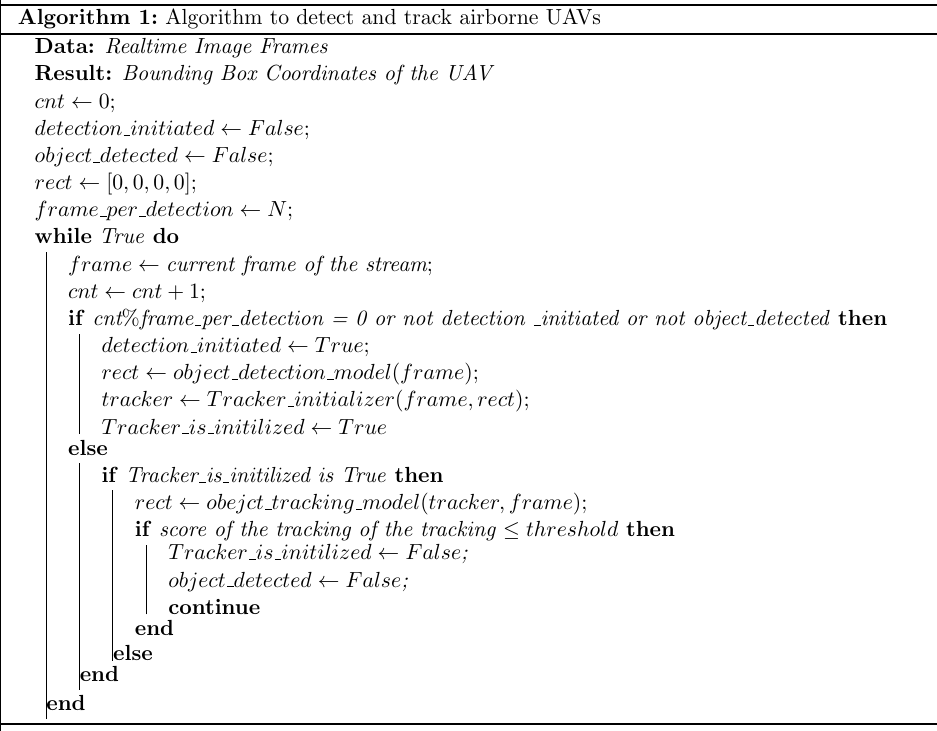
\includegraphics[width=\linewidth]{algo.png}

            \section*{Mission algorithms and control system.}
            The main strategy in the autonomous lockdown algorithm is to select the ideal target, approach the target from behind and lock it, and keep the target within the camera view with vision-based guidance. The steps and related explanations required for this strategy are given under this heading.\\
            For autonomous locking, firstly the target must be approached from the appropriate angle and distance so that the next stage of the mission, vision-based guidance, can be performed. There are two requirements for this approach, which are target selection and path planning. To make the target selection less complicated, the rival UAVs are assumed to be identical and they have the same flight characteristics as the designed vehicle.

            In order for the UAV to approach the target correctly, a path suitable for the flight characteristics must be generated between the current location and the target location\\

            To generate such paths in 3D environments from vector to vector with constraints such as turning and climbing, an improved version of Dubin's path from 2D to 3D, also named Dubins Airplane, is proposed in the following paper[4]. While this work is the reference point for the implementation by our team, it does not exactly match the work of Owen and others. Along with this implementation, which was developed over the vector field methodology, Demirdal’s study is also used as a reference in the developed software [5].

        \end{multicols}
        %% This is needed if you want to add comments in
        %% your algorithm with \Comment

    }
    %----------------------------------------------------------------------------------------
    %	MOTIVATION
    %----------------------------------------------------------------------------------------

    \headerbox{Motivation}{name=motivation,column=1,row=0}{

        The study aims to find a design solution for tracking of mini-class UAVs by a mini-class fixed wing UAV with a camera. The use of mini-class UAVs for civilian or military purposes is gradually increasing \cite{laytonai} and as a result, detection, tracking and destruction of UAVs with potential risk plays an important role. Although this is the main motivation in the design of the designed vehicle system, it is not limited to it. With the increase in the use of unmanned aerial vehicles in the military field, it is expected that UAVs will be included in dogfights \cite{hassanalian2017classifications}. It is aimed to develop a mini-class scale unmanned aerial vehicle that can perform such an operation at a basic level. It is also aimed to develop algorithms to complete such a design.

    }

    %----------------------------------------------------------------------------------------
    %	RESULTS 1
    %----------------------------------------------------------------------------------------

    \headerbox{Results 1}{name=results,column=2,span=1,row=0}{

    }

    %----------------------------------------------------------------------------------------
    %	blank
    %----------------------------------------------------------------------------------------

    \headerbox{blank}{name=references,column=0,above=bottom}{

        Integer sed lectus vel mauris euismod suscipit. Praesent a est a est ultricies pellentesque. Donec tincidunt, nunc in feugiat varius, lectus lectus auctor lorem, egestas molestie risus erat ut nibh.

        Maecenas viverra ligula a risus blandit vel tincidunt est adipiscing. Suspendisse mollis iaculis sem, in \emph{imperdiet} orci porta vitae. Quisque id dui sed ante sollicitudin sagittis.
        \vspace{20em}
    }

    \headerbox{bla2k}{name=reference2,column=0,above=references,below=method}{

        sdsd
    }

    %----------------------------------------------------------------------------------------
    %	References
    %----------------------------------------------------------------------------------------

    \headerbox{References}{name=futureresearch,column=1,span=2,above=bottom}{
        \begin{multicols}{2}
            \renewcommand{\section}[2]{\vskip 0.05em} % Get rid of the default "References" section title
            \nocite{*} % Insert publications even if they are not cited in the poster
            \small{ % Reduce the font size in this block
                \bibliographystyle{unsrt}
                \bibliography{sample} % Use sample.bib as the bibliography file
            }
        \end{multicols}
    }

    %----------------------------------------------------------------------------------------
    %	CONTACT INFORMATION
    %----------------------------------------------------------------------------------------



    %----------------------------------------------------------------------------------------
    %	CONCLUSION
    %----------------------------------------------------------------------------------------

    \headerbox{Conclusion}{name=conclusion,column=2,span=1,row=0,below=results,above=futureresearch}{

        \begin{multicols}{2}

            \tikzstyle{decision} = [diamond, draw, fill=blue!20, text width=4.5em, text badly centered, node distance=2cm, inner sep=0pt]
            \tikzstyle{block} = [rectangle, draw, fill=blue!20, text width=5em, text centered, rounded corners, minimum height=4em]
            \tikzstyle{line} = [draw, -latex']
            \tikzstyle{cloud} = [draw, ellipse, fill=red!20, node distance=3cm, minimum height=2em]

            \begin{tikzpicture}[node distance = 3cm, auto]
                \node [block] (init) {Initialize Model};
                \node [cloud, left of=init] (Start) {Start};
                \node [cloud, right of=init] (Start2) {Start Two};
                \node [block, below of=init] (init2) {Initialize Two};
                \node [decision, below of=init2] (End) {End};
                \path [line] (init) -- (init2);
                \path [line] (init2) -- (End);
                \path [line, dashed] (Start) -- (init);
                \path [line, dashed] (Start2) -- (init);
                \path [line, dashed] (Start2) |- (init2);
            \end{tikzpicture}

            %------------------------------------------------

            \begin{itemize}\compresslist
                \item Pellentesque eget orci eros. Fusce ultricies, tellus et pellentesque fringilla, ante massa luctus libero, quis tristique purus urna nec nibh. Phasellus fermentum rutrum elementum. Nam quis justo lectus.
                \item Vestibulum sem ante, hendrerit a gravida ac, blandit quis magna.
                \item Donec sem metus, facilisis at condimentum eget, vehicula ut massa. Morbi consequat, diam sed convallis tincidunt, arcu nunc.
                \item Nunc at convallis urna. isus ante. Pellentesque condimentum dui. Etiam sagittis purus non tellus tempor volutpat. Donec et dui non massa tristique adipiscing.
            \end{itemize}

        \end{multicols}
    }



    %----------------------------------------------------------------------------------------
    %	RESULTS 2
    %----------------------------------------------------------------------------------------

    \headerbox{Results 2}{name=results2,column=1,below=method,bottomaligned=conclusion}{ % This block's bottom aligns with the bottom of the conclusion block

        Additional recommendations:
        \begin{itemize}\compresslist
            \item Structure your poster by Abstract, Methods, Results and Conclusions.
            \item Every graphic/table should have a caption.
            \item Do not justify blocks of text on both sides.
            \item Highlight your main finding.
            \item If possible, avoid abbreviations and acronyms.
            \item Where possible, express points as bullets rather than paragraphed text.
            \item Use a constant font throughout the poster.
        \end{itemize}


        \textbf{Rule of thumb:}
        The poster is supposed to be readable in screen laptops. Check your final design in full screen.


        \begin{center}
            
\includegraphics[width=0.6\linewidth]{AdımODTÜ_logo.PNG}
            \captionof{figure}{Figure caption}
        \end{center}
    }

    %----------------------------------------------------------------------------------------

\end{poster}

\end{document}